% Part: sets-functions-relations
% Chapter: relations
% Section: trees

\documentclass[../../../include/open-logic-section]{subfiles}

\begin{document}

\olfileid[zh]{sfr}{rel}{tre}
\olsection{树}

一种在逻辑的各个部分中都扮演重要角色的特殊偏序是\emph{树}。有穷树出现在逻辑的初级部分：例如，!!{formula}可以通过它们分解为句法树来理解，而许多!!{derivation}系统中的!!{derivation}也采用有穷树的形式。
%
无穷树已经出现在命题逻辑和一阶逻辑完全性定理的证明中，并广泛用于数理逻辑的各个领域。

树的集合论概念与图论中树的概念密切相关。下面是一棵（有穷）树的图示：

\begin{center}
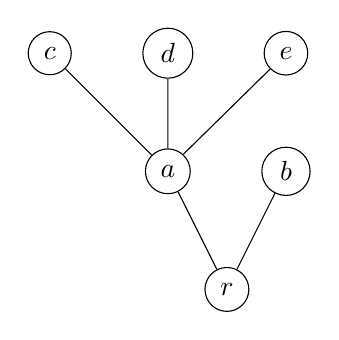
\begin{tikzpicture}[nodes={draw, circle}, -]
\node{$r$} [grow'=up]
    child { node {$a$}
        child { node {$c$} }
        child { node {$d$} }
        child { node {$e$} }
    }
    child { node {$b$} };
\end{tikzpicture}
\end{center}

最底层节点~$r$ 是根。除~$r$ 之外的每个节点在紧邻其下方都恰好有一个父节点。如果从节点~$x$ 沿边向上能够到达节点~$y$，我们可以把 $x$ 与 $y$ 之间的这种关系理解为：$x$ 是~$y$ 的一个\emph{祖先}。

树中的祖先关系构成一个严格偏序。这启发了下面对树的集合论定义。为给出这个定义，我们需要先引入两个概念。设 $\le$ 是集合~$A$ 上的偏序。若!!a{element} $x \in A$ 对任意 $y \in A$ 都满足 $x \le y$，则称 $x$ 为~$A$ 的\emph{最小元}。若~$A$ 的每个非空子集都有最小元，则称 $\le$ 是~$A$ 上的\emph{良序}。

\begin{defn}[树]
一棵\emph{树}是一个二元组 $T = \tuple{A, \le}$，其中 $A$ 是集合，$\le$ 是~$A$ 上的偏序，且具有唯一的最小元 $r \in A$（称为\emph{根}）并且对每个 $x \in A$，$\le$ 在集合 $\Setabs{y}{y \le x}$ 上都是良序。
\end{defn}

\begin{defn}[后继点]
设 $T = \tuple{A, \le}$ 是一棵树。
若 $x,y \in A$，$x < y$，且不存在 $z \in A$ 使 $x < z < y$，则称 $y$ 是~$x$ 的一个\emph{后继}。
\end{defn}

$x \in A$ 的后继也称为它的\emph{子节点}。若 $y$ 是~$x$ 的一个后继，则称 $x$ 为~$y$ 的\emph{前驱点}或\emph{父节点}。

\begin{prop}
若 $\tuple{A,\le}$ 是一棵树，则除根之外的每个 $x \in A$ 至多有一个前驱点。
\end{prop}

\begin{proof}
  设 $y_1 < x$ 且 $y_2 < x$ 且 $y_1 \neq y_2$。则 $\{y_1,
  y_2\} \subseteq \Setabs{z}{z<x}$。由于 $\Setabs{z}{z<x}$ 在 $\le$ 下是良序，其子集 $\{y_1, y_2\}$ 有一个最小元，显然它必须是 $y_1$ 或~$y_2$。所以要么 $y_1 \le y_2$，要么 $y_2 \le y_1$。我们假设了 $y_1 \neq y_2$，因此实际上要么 $y_1 < y_2$，要么 $y_2 < y_1$。由于我们假设了 $y_1 < x$ 和 $y_2 < x$，我们进而有要么 $y_1 < y_2
  < x$，要么 $y_2 < y_1 < x$。所以 $y_1$ 和 $y_2$ 不可能都是~$x$ 的前驱点。
\end{proof}

\begin{defn}
若 $A$ 是无穷集合，则称树 $T = \tuple{A, \le}$ 是\emph{无穷的}，否则称它是\emph{有穷的}。若 $T$ 使得每个 $x \in A$ 只有有穷多个后继，则称 $T$ 是\emph{有穷分支的}。
\end{defn}

\begin{defn}[支]
给定一棵树 $T = \tuple{A, \le}$，$T$ 的一个\emph{支}是~$T$ 中的极大链，即一个集合 $B \subseteq A$，使得对任意 $x, y \in B$ 要么 $x \le y$ 要么 $y \le x$，且对任意 $z \in A \setminus B$ 存在 $u \in B$ 使得既非 $z \le u$ 也非 $u \le z$。
%
用 $[T]$ 表示 $T$ 的所有支的集合。
\end{defn}

\begin{ex}
有穷分支树的一个经典例子是由 $0$ 和~$1$ 的有穷序列构成的\emph{无穷二叉树}，有时记为 $\{0,1\}^*$ 或~$\Bin^*$，按扩展关系 $\sqsubseteq$ 排序（例如 $101 \sqsubseteq 101101$）。由于任何二进制串总可以在末尾添加一个 $0$ 或一个 $1$ 来扩展，这棵树包含无穷多个元素：每个元素~$s$ 恰好有两个后继，$s0$ 和~$s1$。它的根是空序列 $\emptyseq$。
\end{ex}

\begin{ex}
稍微一般地说，自然数的有穷序列的集合~$\Nat^*$ 连同扩展关系~$\sqsubseteq$ 也是一棵树。它显然不是有穷分支的：每个 $s \in \Nat^*$ 都有无穷多个后继~$sn$，对每个 $n \in \Nat$ 各有一个。每个对~$\sqsubseteq$ 封闭的 $A
\subseteq \Nat^*$ 都是~$\Nat^*$ 的一个\emph{子树}。（也就是说，$A$ 满足若 $s \in A$ 且 $s' \sqsubseteq s$，则也有 $s' \in A$。）所有有穷树都可以表示为~$\Nat^*$ 的有穷子树。
\end{ex}

\begin{prop}[K\H{o}nig 引理]
若 $T = \tuple{A,\le}$ 是一棵有穷分支的无穷树，则 $T$ 有一个无穷支。
\end{prop}

K\H{o}nig 引理的一个在可计算性理论中广泛使用的特殊情形，称为\emph{弱 K\H{o}nig 引理}，如下：$\{0,1\}^*$ 的任何无穷子树都有一个无穷支。

\end{document}
